\documentclass{article}
%\documentstyle[11pt,handout,psfig]{article}

\usepackage{fullpage,amssymb,amsmath,tikz,forest,float,subcaption,braket}
\usetikzlibrary{arrows.meta}

\forestset{
    default preamble={
        for tree={
        	   font=\tiny,
            base=bottom,
            child anchor=north,
            align=center,
            s sep+=1.3cm,
    straight edge/.style={
        edge path={\noexpand\path[\forestoption{edge},thick,-{Latex}] 
        (!u.parent anchor) -- (.child anchor);}
    },
    if n children={0}
        {tier=word, draw, thick, rectangle}
        {
        		if n children={1}
        		{draw, thick, rectangle, parent anchor=south}
        		{draw, diamond, thick, aspect=2}
        },
    if n=1{%
    		if n'=1
    			{edge path={\noexpand\path[\forestoption{edge},thick,-{Latex}] 
        			(!u.parent anchor) -| (.child anchor);}}
        		{edge path={\noexpand\path[\forestoption{edge},thick,-{Latex}] 
        			(!u.parent anchor) -| (.child anchor) node[pos=.2, above] {Y};}}
        }{
        edge path={\noexpand\path[\forestoption{edge},thick,-{Latex}] 
        (!u.parent anchor) -| (.child anchor) node[pos=.2, above] {N};}
        }
        }
    }
}

\usepackage[12pt]{extsizes}
\usepackage{gensymb}
\usepackage{graphicx}




%These give really tight margins:
%\setlength{\topmargin}{-0.3in}
%\setlength{\textheight}{8.10in}
%\setlength{\textwidth}{5.8in}
%\setlength{\baselineskip}{0.1875in}
%\addtolength{\leftmargin}{-2.775in}
%\setlength{\footskip}{0.45in}
%\setlength{\oddsidemargin}{0.5in}
%\setlength{\evensidemargin}{0.5in}
%%\setlength{\headsep}{0pt}
%%\setlength{\headheight}{0pt}

%\setlength{\topmargin}{-0.5in}
\setlength{\textheight}{8in}
%\setlength{\textwidth}{5.0in}
%\setlength{\baselineskip}{0.1875in}
%\addtolength{\leftmargin}{-2.775in}
%\setlength{\footskip}{0.45in}
%\setlength{\oddsidemargin}{0.5in}
%\setlength{\evensidemargin}{0.5in}
%%\setlength{\headsep}{0pt}
%%\setlength{\headheight}{0pt}


\markright{XCS229i}
\pagestyle{myheadings}

\newcommand{\newsec}{\section}
\newcommand{\denselist}{\itemsep 0pt\partopsep 0pt}
\newcommand{\bitem}{\begin{itemize}\denselist}
\newcommand{\eitem}{\end{itemize}}
\newcommand{\benum}{\begin{enumerate}\denselist}
\newcommand{\eenum}{\end{enumerate}}

\newcommand{\fig}[1]{\private{\begin{center}
{\Large\bf ({#1})}
\end{center}}}

\newcommand{\cpsf}[1]{{\centerline{\psfig{#1}}}}
\newcommand{\mytitle}[1]{\centerline{\LARGE\bf #1}}

\newcommand{\myw}{{\bf w}}

\newcommand{\mypar}[1]{\vspace{1ex}\noindent{\bf {#1}}}

\def\thmcolon{\hspace{-.85em} {\bf :} }

\newtheorem{THEOREM}{Theorem}[section]
\newenvironment{theorem}{\begin{THEOREM} \thmcolon }%
                        {\end{THEOREM}}
\newtheorem{LEMMA}[THEOREM]{Lemma}
\newenvironment{lemma}{\begin{LEMMA} \thmcolon }%
                      {\end{LEMMA}}
\newtheorem{COROLLARY}[THEOREM]{Corollary}
\newenvironment{corollary}{\begin{COROLLARY} \thmcolon }%
                          {\end{COROLLARY}}
\newtheorem{PROPOSITION}[THEOREM]{Proposition}
\newenvironment{proposition}{\begin{PROPOSITION} \thmcolon }%
                            {\end{PROPOSITION}}
\newtheorem{DEFINITION}[THEOREM]{Definition}
\newenvironment{definition}{\begin{DEFINITION} \thmcolon \rm}%
                            {\end{DEFINITION}}
\newtheorem{CLAIM}[THEOREM]{Claim}
\newenvironment{claim}{\begin{CLAIM} \thmcolon \rm}%
                            {\end{CLAIM}}
\newtheorem{EXAMPLE}[THEOREM]{Example}
\newenvironment{example}{\begin{EXAMPLE} \thmcolon \rm}%
                            {\end{EXAMPLE}}
\newtheorem{REMARK}[THEOREM]{Remark}
\newenvironment{remark}{\begin{REMARK} \thmcolon \rm}%
                            {\end{REMARK}}
%\newenvironment{proof}{\noindent {\bf Proof:} \hspace{.677em}}%
%                      {}

%theorem
\newcommand{\thm}{\begin{theorem}}
%lemma
\newcommand{\lem}{\begin{lemma}}
%proposition
\newcommand{\pro}{\begin{proposition}}
%definition
\newcommand{\dfn}{\begin{definition}}
%remark
\newcommand{\rem}{\begin{remark}}
%example
\newcommand{\xam}{\begin{example}}
%corollary
\newcommand{\cor}{\begin{corollary}}
%proof
\newcommand{\prf}{\noindent{\bf Proof:} }
%end theorem
\newcommand{\ethm}{\end{theorem}}
%end lemma
\newcommand{\elem}{\end{lemma}}
%end proposition
\newcommand{\epro}{\end{proposition}}
%end definition
\newcommand{\edfn}{\bbox\end{definition}}
%end remark
\newcommand{\erem}{\bbox\end{remark}}
%end example
\newcommand{\exam}{\bbox\end{example}}
%end corollary
\newcommand{\ecor}{\end{corollary}}
%end proof
\newcommand{\eprf}{\bbox\vspace{0.1in}}
%begin equation
\newcommand{\beqn}{\begin{equation}}
%end equation
\newcommand{\eeqn}{\end{equation}}

%\newcommand{\eqref}[1]{Eq.~\ref{#1}}

\newcommand{\KB}{\mbox{\it KB\/}}
\newcommand{\infers}{\vdash}
\newcommand{\sat}{\models}
\newcommand{\bbox}{\vrule height7pt width4pt depth1pt}

\newcommand{\act}[1]{\stackrel{{#1}}{\rightarrow}}
\newcommand{\at}[1]{^{(#1)}}

\newcommand{\argmax}{{\rm argmax}}
\newcommand{\V}{{\cal V}}
\newcommand{\C}{{\cal C}}
\newcommand{\calL}{{\cal L}}

\newcommand{\rimp}{\Rightarrow}
\newcommand{\dimp}{\Leftrightarrow}

\newcommand{\nf}{\bar{f}}
\newcommand{\ns}{\bar{s}}
\newcommand{\na}{\bar{a}}
\newcommand{\nh}{\bar{h}}
\newcommand{\nr}{\bar{r}}


\newcommand{\bX}{\mbox{\boldmath $X$}}
\newcommand{\bY}{\mbox{\boldmath $Y$}}
\newcommand{\bZ}{\mbox{\boldmath $Z$}}
\newcommand{\bU}{\mbox{\boldmath $U$}}
\newcommand{\bE}{\mbox{\boldmath $E$}}
\newcommand{\bx}{\mbox{\boldmath $x$}}
\newcommand{\be}{\mbox{\boldmath $e$}}
\newcommand{\by}{\mbox{\boldmath $y$}}
\newcommand{\bz}{\mbox{\boldmath $z$}}
\newcommand{\bu}{\mbox{\boldmath $u$}}
\newcommand{\bd}{\mbox{\boldmath $d$}}
\newcommand{\smbx}{\mbox{\boldmath $\scriptstyle x$}}
\newcommand{\smbd}{\mbox{\boldmath $\scriptstyle d$}}
\newcommand{\smby}{\mbox{\boldmath $\scriptstyle y$}}
\newcommand{\smbe}{\mbox{\boldmath $\scriptstyle e$}}

\newcommand{\Parents}{\mbox{\it Parents\/}}
\newcommand{\B}{{\cal B}}

\newcommand{\word}[1]{\mbox{\it #1\/}}
\newcommand{\Action}{\word{Action}}
\newcommand{\Proposition}{\word{Proposition}}
\newcommand{\true}{\word{true}}
\newcommand{\false}{\word{false}}
\newcommand{\Pre}{\word{Pre}}
\newcommand{\Add}{\word{Add}}
\newcommand{\Del}{\word{Del}}
\newcommand{\Result}{\word{Result}}
\newcommand{\Regress}{\word{Regress}}
\newcommand{\Maintain}{\word{Maintain}}

\newcommand{\bor}{\bigvee}
\newcommand{\invert}[1]{{#1}^{-1}}

\newcommand{\commentout}[1]{}

\newcommand{\bmu}{\mbox{\boldmath $\mu$}}
\newcommand{\btheta}{\mbox{\boldmath $\theta$}}
\newcommand{\IR}{\mbox{$I\!\!R$}}

\newcommand{\tval}[1]{{#1}^{1}}
\newcommand{\fval}[1]{{#1}^{0}}

\newcommand{\tr}{{\rm tr}}
\newcommand{\vecy}{{\vec{y}}}
\renewcommand{\Re}{{\mathbb R}}

\def\twofigbox#1#2{%
\noindent\begin{minipage}{\textwidth}%
\epsfxsize=0.35\maxfigwidth
\noindent \epsffile{#1}\hfill
\epsfxsize=0.35\maxfigwidth
\epsffile{#2}\\
\makebox[0.35\textwidth]{(a)}\hfill\makebox[0.35\textwidth]{(b)}%
\end{minipage}}

\def\twofigboxcd#1#2{%
\noindent\begin{minipage}{\textwidth}%
\epsfxsize=0.35\maxfigwidth
\noindent \epsffile{#1}\hfill
\epsfxsize=0.35\maxfigwidth
\epsffile{#2}\\
\makebox[0.35\textwidth]{(c)}\hfill\makebox[0.35\textwidth]{(d)}%
\end{minipage}}

\def\twofigboxnolabel#1#2{%
\begin{figure}[h]
\centering
\begin{minipage}{.5\textwidth}
  \centering
  \includegraphics[width=0.75\linewidth]{#1}
\end{minipage}%
\begin{minipage}{.5\textwidth}
  \centering
  \includegraphics[width=0.75\linewidth]{#2}
\end{minipage}
\end{figure}
}

\def\threefigbox#1#2#3{%
\noindent\begin{minipage}{\textwidth}%
\epsfxsize=0.33\maxfigwidth
\noindent \epsffile{#1}\hfill
\epsfxsize=0.33\maxfigwidth
\noindent \epsffile{#2}\hfill 
\epsfxsize=0.33\maxfigwidth
\epsffile{#3}\\
\makebox[0.31\textwidth]{{\scriptsize (a)}}\hfill%
\makebox[0.31\textwidth]{{\scriptsize (b)}}\hfill
\makebox[0.31\textwidth]{{\scriptsize (c)}}%
\smallskip
\end{minipage}}


\def\threefigbox#1#2#3{%
\begin{figure}[H]
\centering
\begin{subfigure}{.33\textwidth}
  \centering
  \includegraphics[width=0.75\linewidth]{#1}
  \caption{}
\end{subfigure}%
\begin{subfigure}{.33\textwidth}
  \centering
  \includegraphics[width=0.75\linewidth]{#2}
   \caption{}
\end{subfigure}%
\begin{subfigure}{.33\textwidth}
  \centering
  \includegraphics[width=0.75\linewidth]{#3}
   \caption{}
\end{subfigure}
\end{figure}
}


\def\threefigboxnolabel#1#2#3{%
\centering
\begin{subfigure}{.33\textwidth}
  \centering
  \includegraphics[width=0.75\linewidth]{#1}
\end{subfigure}%
\begin{subfigure}{.33\textwidth}
  \centering
  \includegraphics[width=0.75\linewidth]{#2}
\end{subfigure}%
\begin{subfigure}{.33\textwidth}
  \centering
  \includegraphics[width=0.75\linewidth]{#3}
\end{subfigure}
\end{figure}
}

\newlength{\maxfigwidth}
\setlength{\maxfigwidth}{\textwidth}
%\def\captionsize {\footnotesize}
\def\captionsize {}

\newcommand{\xsi}{{x^{(i)}}}
\newcommand{\ysi}{{y^{(i)}}}
\newcommand{\wsi}{{w^{(i)}}}
\newcommand{\esi}{{\epsilon^{(i)}}}
\newcommand{\calN}{{\cal N}}
\newcommand{\calX}{{\cal X}}
\newcommand{\calY}{{\cal Y}}
\newcommand{\ytil}{{\tilde{y}}}

\newcommand{\beas}{\begin{eqnarray*}}
\newcommand{\eeas}{\end{eqnarray*}}

\newcommand{\Ber}{{\rm Bernoulli}}
\newcommand{\Bernoulli}{{\rm Bernoulli}}
\newcommand{\E}{{\rm E}}

\begin{document}
\title{XCS229i Lecture Notes}
\author{Andrew Ng}
\date{}
\maketitle


\part*{Decision Trees}

We now turn our attention to decision trees, a simple yet flexible class of algorithms.  We will first consider the non-linear, region-based nature of decision trees, continue on to define and contrast region-based loss functions, and close off with an investigation of some of the specific advantages and disadvantages of such methods.  Once finished with their nuts and bolts, we will move on to investigating different ensembling methods through the lens of decision trees, due to their suitability for such techniques.  

\section{Non-linearity}

Importantly, decision trees are one of the first inherently {\bf non-linear} machine learning techniques we will cover, as compared to methods such as vanilla SVMs or GLMs.  Formally, a method is linear if for an input $x \in \mathbb{R}^n$ (with interecept term $x_0 = 1$) it only produces hypothesis functions $h$ of the form:

$$h(x) = \theta^T x$$

where $\theta \in \mathbb{R}^n$.  Hypothesis functions that cannot be reduced to the form above are called non-linear, and if a method can produce non-linear hypothesis functions then it is also non-linear.  We have already seen that kernelization of a linear method is one such method by which we can achieve non-linear hypothesis functions, via a feature mapping $\phi(x)$.

Decision trees, on the other hand, can directly produce non-linear hypothesis functions without the need for first coming up with an appropriate feature mapping.  As a motivating (and very Canadien) example, let us say we want to build a classifier that, given a time and a location, can predict whether or not it would be possible to ski nearby.  To keep things simple, the time is represented as month of the year and the location is represented as a latitude (how far North or South we are with $-90\degree$, $0\degree$, and $90\degree$ being the South Pole, Equator, and North Pole, respectively). 

\twofigboxnolabel{ski.eps}{ski-region.eps}


A representative dataset is shown above left.  There is no linear boundary that would correctly split this dataset.  However, we can recognize that there are different areas of positive and negative space we wish to isolate, one such division being shown above right.  We accomplish this by partitioning the input space $\mathcal{X}$ into disjoint subsets (or {\bf regions}) $R_i$:

\begin{align*}
\mathcal{X} & = \bigcup\limits_{i=0}^{n} R_i\\
\text{s.t.}\qquad R_i   \cap R_j &= \emptyset \enskip \text{for} \enskip i \neq j
\end{align*}

where $n \in \mathbb{Z}^+$.

\section{Selecting Regions}
\label{Regions}

In general, selecting optimal regions is intractable.  Decision trees generate an approximate solution via {\bf greedy, top-down, recursive partitioning}.  The method is {\bf top-down} because we start with the original input space $\mathcal{X}$ and split it into two child regions by thresholding on a single feature.  We then take one of these child regions and can partition via a new threshold.  We continue the training of our model in a {\bf recursive} manner, always selecting a leaf node, a feature, and a threshold to form a new split.  Formally, given a parent region $R_p$, a feature index $j$, and a threshold $t  \in \mathbb{R}$, we obtain two child regions $R_1$ and $R_2$ as follows:

\begin{align*}
R_1 = \{ X \mid X_j < t, X \in R_p \}\\
R_2 = \{ X \mid X_j \geq t, X \in R_p \}
\end{align*}

The beginning of one such process is shown below applied to the skiing dataset.  In step \subref{fig:step1}, we split the input space $\mathcal{X}$ by the location feature, with a threshold of 15, creating child regions $R_1$ and $R_2$.  In step \subref{fig:step2}, we then recursively select one of these child regions (in this case $R_2$) and select a feature (time) and threshold ($3$), generating two more child regions ($R_{21}$ and $R_{22}$).  In step \subref{fig:step3}, we select any one of the remaining leaf nodes ($R_1$, $R_{21}$, $R_{22}$).  We can continue in such a manner until we a meet a given stop criterion (more on this later), and then predict the majority class at each leaf node. 


\begin{figure}[H]
\centering

\begin{subfigure}[t]{\textwidth}
	\centering
	\begin{minipage}[t]{.35\linewidth}
		\centering
		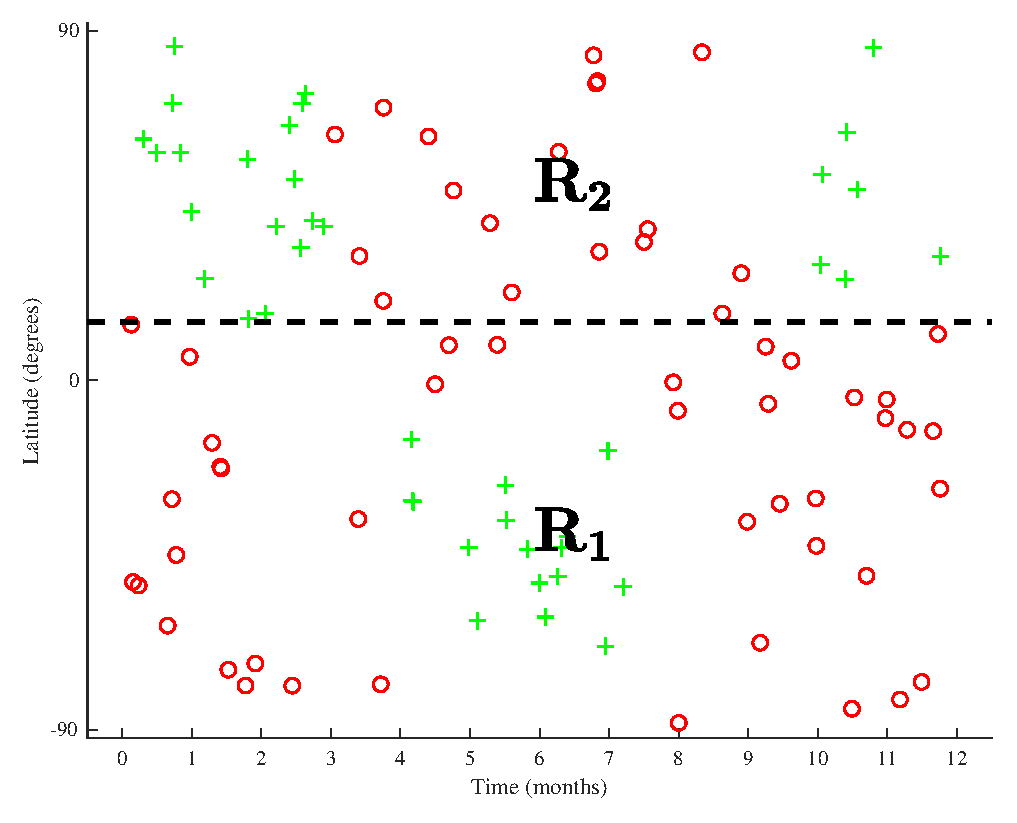
\includegraphics[width=\linewidth]{ski-split1.eps}
		\caption{}
		\label{fig:step1}
	\end{minipage}
	\begin{minipage}[t]{.6\linewidth}
		\qquad
		\begin{forest}
		[$\text{loc} < 15$, tikz={\draw[{Latex}-, thick] (.north) --++ (0,1);}
	    		[$R_1$]
	    		[$R_2$] 
		] 
		\end{forest}
	\end{minipage}
\end{subfigure}

\begin{subfigure}[t]{\textwidth}
	\centering
	\begin{minipage}[t]{.35\linewidth}
		\centering
		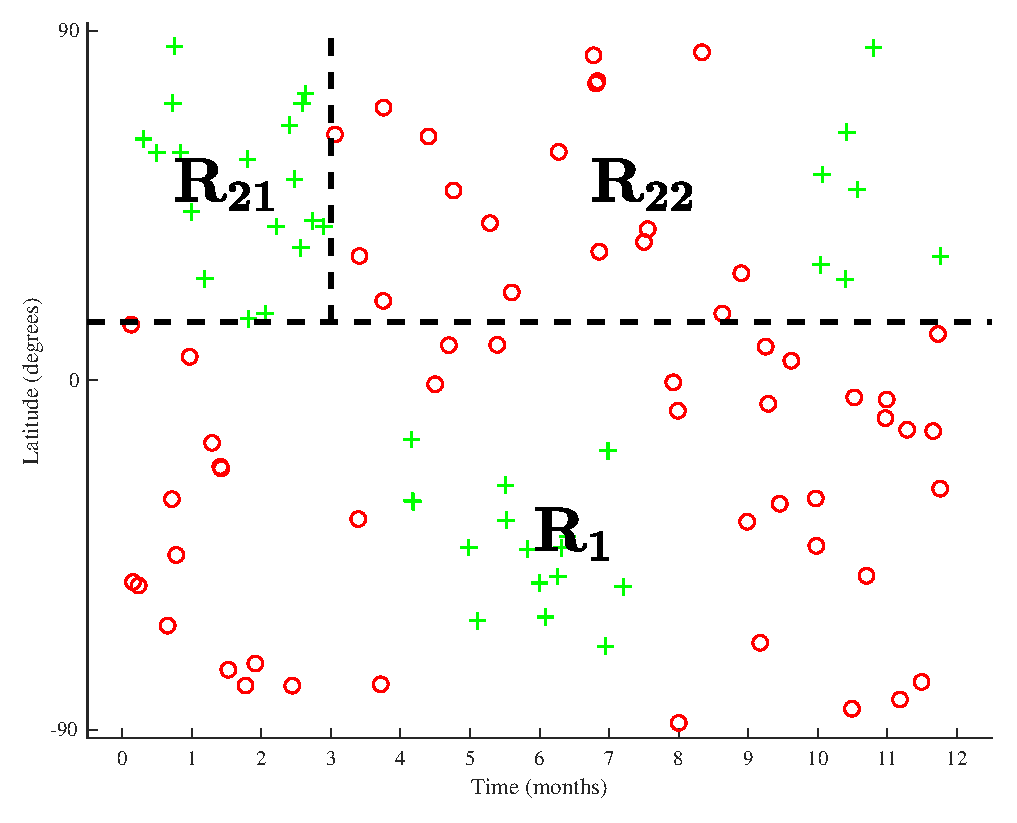
\includegraphics[width=\linewidth]{ski-split2.eps}
		\caption{}
		\label{fig:step2}
	\end{minipage}
	\begin{minipage}[t]{.6\linewidth}
		\qquad
		\begin{forest}
		[$\text{loc} < 15$, tikz={\draw[{Latex}-, thick] (.north) --++ (0,1);}
    			[$R_1$]
    			[$\text{time} < 3$
        			[$R_{21}$] 
        			[$R_{22}$]   
    			]   
		] 
		\end{forest}
	\end{minipage}
\end{subfigure}



\begin{subfigure}[t]{\textwidth}
	\centering
	\begin{minipage}[t]{.35\linewidth}
		\centering
		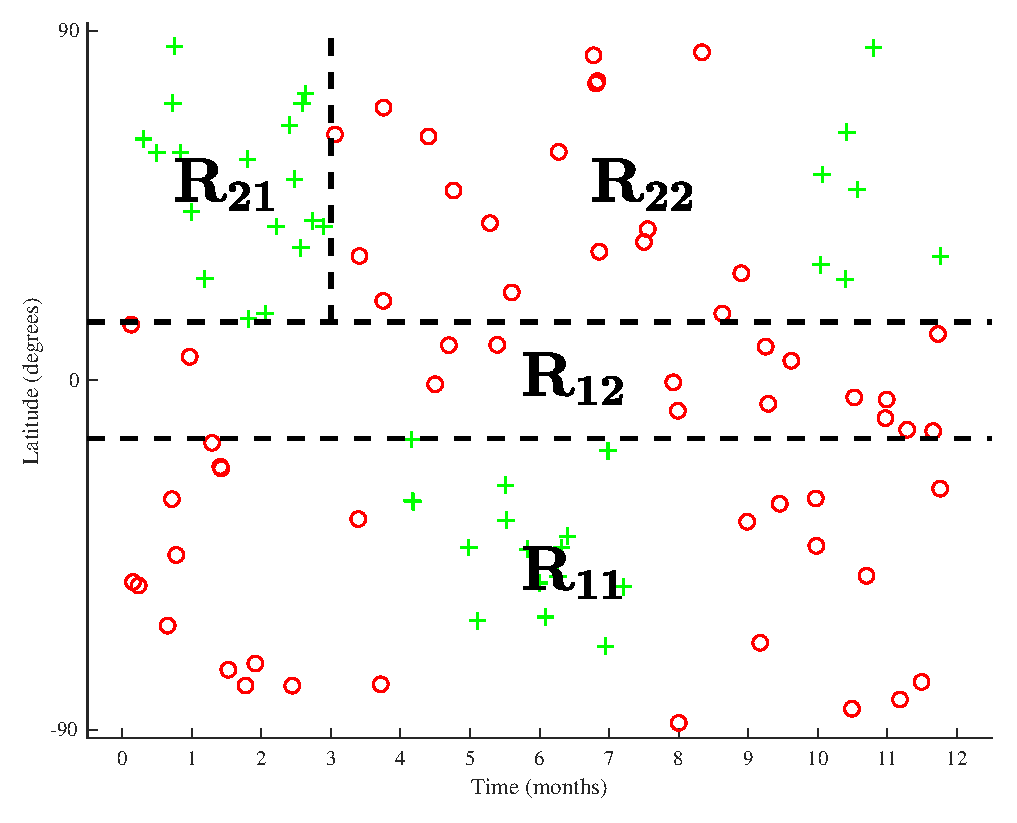
\includegraphics[width=\linewidth]{ski-split3.eps}
		\caption{}
		\label{fig:step3}
	\end{minipage}
	\begin{minipage}[t]{.6\linewidth}
		\qquad
		\begin{forest}
		[$\text{loc} < 15$, tikz={\draw[{Latex}-, thick] (.north) --++ (0,1);}
    			[$\text{loc} < -15$
            			[$R_{11}$] 
           		 	[$R_{12}$] 
        		]   
   			[$\text{time} < 3$
        			[$R_{21}$] 
        			[$R_{22}$]  
   			]   
		] 
		\end{forest}
	\end{minipage}
\end{subfigure}
\end{figure}

\section{Defining a Loss Function}

A natural question to ask at this point is how to choose our splits.  To do so, it is first useful to define our loss $L$ as a set function on a region $R$.  Given a split of a parent $R_p$ into two child regions $R_1$ and $R_2$, we can compute the loss of the parent $L(R_p)$ as well as the cardinality-weighted loss of the children $\frac{|R_1| L(R_1) + |R_2| L(R_2)}{|R_1| + |R_2|}$.  Within our {\bf greedy} partitioning framework, we want to select the leaf region, feature, and threshold that will maximize our decrease in loss:

$$L(R_p) - \frac{|R_1| L(R_1) + |R_2| L(R_2)}{|R_1| + |R_2|}$$

For a classification problem, we are interested in the {\bf misclassification loss} $L_{misclass}$.  For a region $R$ let $\hat{p}_c$ be the proportion of examples in $R$ that are of class $c$.  Misclassification loss on $R$ can be written as:

$$L_{misclass}(R) = 1 - \max_{c}(\hat{p}_c)$$

We can understand this as being the number of examples that would be misclassified if we predicted the majority class for region $R$ (which is exactly what we do).  While misclassification loss is the final value we are interested in, it is not very sensitive to changes in class probabilities.  As a representative example, we show a binary classification case below.  We explicitly depict the parent region $R_p$ as well as the positive and negative counts in each region. 

\begin{figure}[H]
\centering
\begin{minipage}[t]{.45\linewidth}
		\centering
	\begin{forest}
	[$R_p$: 400 + / 100 -,
		[split
			[$R_1$: 150 + / 100 -]
			[$R_2$: 250 + / 0 -]
		]
	] 
	\end{forest}
\end{minipage}
\begin{minipage}[t]{.45\linewidth}
		\centering
	\begin{forest}
	[$R_p$: 400 + / 100 -,
		[split
			[$R_1'$: 300 + / 100 -]
			[$R_2'$: 100 + / 0 -]
		]
	] 
	\end{forest}
\end{minipage}
\end{figure}


 
 The first split is isolating out more of the positives, but we note that:

 $$L(R_p) = \frac{|R_1| L(R_1) + |R_2| L(R_2)}{|R_1| + |R_2|} = \frac{|R_1'| L(R_1') + |R_2'| L(R_2')}{|R_1' + |R_2'|} = 100 $$.
 
  Thus, not only can we not only are the losses of the two splits identical, but neither of the splits decrease the loss over that of the parent.
 
 We therefore are interested in defining a more sensitive loss.  While several have been proposed, we will focus here on the {\bf cross-entropy} loss $L_{cross}$:
 
 $$L_{cross}(R) = - \sum_{c} \hat{p}_c \log_2 \hat{p}_c$$
 
 With $\hat{p} \log_2 \hat{p} \equiv 0$ if $\hat{p} = 0$.  From an information-theoretic perspective, cross-entropy measure the number of bits needed to specify the outcome (or class) given that the distribution is known.  Furthermore, the reduction in loss from parent to child is known as information gain.
 
 To understand the relative sensitivity of cross-entropy loss with respect to misclassification loss, let us look at plots of both loss functions for the binary classification case.  For these cases, we can simplify our loss functions to depend on just the proportion of positive examples $\hat{p}_i$ in a region $R_i$: 
 \begin{align*}
&L_{misclass}(R) = L_{misclass}(\hat{p}) = 1 - \max(\hat{p}, 1 - \hat{p})\\
&L_{cross}(R) = L_{cross}(\hat{p}) = - \hat{p} \log{\hat{p}} - (1 - \hat{p}) \log{(1 - \hat{p})}
 \end{align*}
 
 \twofigboxnolabel{crossentropy.eps}{misclass.eps}
 
 In the figure above on the left, we see the cross-entropy loss plotted over $\hat{p}$.  We take the regions ($R_p$, $R_1$, $R_2$) from the previous page's example's first split, and plot their losses as well.  As cross-entropy loss is strictly concave, it can be seen from the plot (and easily proven) that as long as $\hat{p}_1 \neq \hat{p}_2$ and both child regions are non-empty, then the weighted sum of the children losses will always be less than that of the parent.
 
 Misclassification loss, on the other hand, is not strictly concave, and therefore there is no guarantee that the weighted sum of the children will be less than that of the parent, as shown above right, with the same partition.  Due to this added sensitivity, cross-entropy loss (or the closely related Gini loss) are used when growing decision trees for classification.
 
Before fully moving away from loss functions, we briefly cover the regression setting for decision trees.  For each data point $x_i$ we now instead have an associated value $y_i \in \mathbb{R}$ we wish to predict.  Much of the tree growth process remains the same, with the differences being that the final prediction for a region $R$ is the mean of all the values:

$$\hat{y} = \frac{\sum_{i \in R} y_i}{|R|}$$

And in this case we can directly use the {\bf squared loss} to select our splits:

$$L_{squared}(R) = \frac{\sum_{i \in R} (y_i - \hat{y})^2}{|R|}$$

\section{Other Considerations}

The popularity of decision trees can in large part be attributed to the ease by which they are explained and understood, as well as the high degree of interpretability they exhibit: we can look at the generated set of thresholds to understand why a model made specific predictions.  However, that is not the full picture -- we will now cover some additional salient points.

\subsection{Categorical Variables}

Another advantage of decision trees is that they can easily deal with categorical variables.  As an example, our location in the skiing dataset could instead be represented as a categorical variable (one of Northern Hemisphere, Southern Hemisphere, or Equator (i.e. $\text{loc} \in \{ N, S, E\}$)).  Rather than use a one-hot encoding or similar preprocessing step to transform the data into a quantitative feature, as would be necessary for the other algorithms we have seen, we can directly probe subset membership.   The final tree in Section \ref{Regions} can be re-written as:

\begin{figure}[H]
\centering
\begin{forest}
[$\text{loc} \in \set{S, E}$, tikz={\draw[{Latex}-, thick] (.north) --++ (0,1);}
	[$\text{loc} \in \set{S}$
    			[$R_{11}$] 
   		 	[$R_{12}$] 
		]   
	[$\text{time} < 3$
			[$R_{21}$] 
			[$R_{22}$]  
	]   
] 
\end{forest}
\end{figure}

A caveat to the above is that we must take care to not allow a variable to have too many categories.  For a set of categories $S$, our set of possible questions is the power set $\mathcal{P}(S)$, of cardinality $2^{|S|}$.  Thus, a large number of categories makes question selectioin computationally intractable.  Optimizations are possible for the binary classification, though even in this case serious consideration should be given to whether the feature can be re-formulated as a quantitative one instead as the large number of possible thresholds lend themselves to a high degree of overfitting.

\subsection{Regularization}

In Section \ref{Regions} we alluded to various stopping criteria we could use to determine when to halt the growth of a tree.  The simplest criteria involves "fully" growning the tree: we continue until each leaf region contains exactly one training data point.  This technique however leads to a high variance and low bias model, and we therefore turn to various stopping heuristics for regularization.  Some common ones include:

\begin{itemize}
	\item {\bf Minimum Leaf Size} -- Do not split $R$ if its cardinality falls below a fixed threshold.
	\item {\bf Maximum Depth} -- Do not split $R$ if more than a fixed threshold of splits were already taken to reach $R$.
	\item {\bf Maximum Number of Nodes} -- Stop if a tree has more than a fixed threshold of leaf nodes.
\end{itemize}

A tempting heuristic to use would be to enforce a minimum decrease in loss after splits.  This is a problematic approach as the greedy, single-feature at a time approach of decision trees could mean missing higher order interactions.  If we require thresholding on multiple features to achieve a good split, we might be unable to achieve a good decrease in loss on the initial splits and therefore prematurely terminate.  A better approach involves fully growing out the tree, and then pruning away nodes that minimally decrease misclassification or squared error, as measured on a validation set. 

\subsection{Runtime}

We briefly turn to considering the runtime of decision trees.  For ease of analysis, we will consider binary classification with $n$ examples, $f$ features, and a tree of depth $d$.   At test time, for a data point we traverse the tree until we reach a leaf node and then output its prediction, for a runtime of $O(d)$.  Note that if our tree is balanced than $d = O(\log{n})$, and thus test time performance is generally quite fast.

At training time, we note that each data point can only appear in at most $O(d)$ nodes.  Through sorting and intelligent caching of intermediate values, we can achieve an amortized runtime of $O(1)$ at each node for a single data point for a single feature.  Thus, overall runtime is $O(nfd)$ -- a fairly fast runtime as the data matrix alone is of size $nf$.

\subsection{Lack of Additive Structure}

One important downside to consider is that decision trees can not easily capture additive structure.  For example, as seen below on the left, a simple decision boundary of the form $x_1 + x_2$ could only be approximately modeled through the use of many splits, as each split can only consider one of $x_1$ or $x_2$ at a time.  A linear model on the other hand could directly derive this boundary, as shown below right.

 \twofigboxnolabel{additive_dt.eps}{additive_linear.eps}

While there has been some work in allowing for decision boundaries that factor in many features at once, they have the downside of further increasing variance and reducing interpretability.
 
\pagebreak 
 
\section{Recap}

To summarize, some of the primary benefits of decision trees are:

\begin{itemize}
	\item[$+$] Easy to explain
	\item[$+$] Interpretable
	\item[$+$] Categorical variable support
	\item[$+$]Fast
\end{itemize}

While some of the disadvantages include:

\begin{itemize}
	\item[$-$] High variance
	\item[$-$] Poor additive modeling
\end{itemize}

Unfortunately, these problems tend to cause individual decision trees to have low overall predictive accuracy.  A common (and successful) way to address these issues is through ensembling methods -- our next topic of discussion.

\end{document}
